%====================================================================
\frame{ \frametitle{Joint, Marginal, Conditional (1/2)} \label{app:JointMargCond}

  \paragraph{Reminder:} 2 loci with 2 alleles each: $(A, a)$, $(B, b)$
  \begin{itemize}
   \item Joint distribution: 
   $$
   \begin{array}{c|cc|c}
   & B & b & \text{marginal} \\
   \hline
   A & f_{AB} & f_{Ab} & p_A = f_{AB} + f_{Ab} \\
   a & f_{aB} & f_{ab} & p_a = f_{aB} + f_{ab} \\
   \hline
   \text{marginal} & q_B = f_{AB} + f_{aB} & q_b = f_{Ab} + f_{ab} & 
    f_{AB} + f_{Ab} + f_{aB} + f_{ab} = 1 
  \end{array}
  $$ \\ ~
  \item Marginal distribution: 'integrate out' the allele of the other locus
  $$
  \Pr\{B\} = q_B = f_{AB} + f_{aB}
  $$ \\ ~
  \item Conditional distribution: fix the allele of the other locus
  $$
  \Pr\{A \gv b\} = \frac{\Pr\{A, b\}}{\Pr\{b\}} = \frac{f_{Ab}}{q_b} = \frac{f_{Ab}}{f_{Ab} + f_{ab}}
  $$
  \end{itemize}
}

%====================================================================
\frame{ \frametitle{Joint, Marginal, Conditional (2/2)} \label{app:JointMargCond}

  \paragraph{Continuous case:} 2 continuous random variables $X$ and $Y$
  \begin{itemize}
   \item Joint distribution: 
   $$
   \begin{array}{c|c|c}
   & y  & \text{marginal} \\
   \hline
   x & p_{XY}(x, y) & p_X(x) = \int p_{XY}(x, y) \d y \\
   \hline
   \text{marginal} & p_Y(y) = \int p_{XY}(x, y) \d x & \int p_{XY}(x, y) \d x \d y = 1 
   \end{array}
  $$ \\ ~
  \item Marginal distribution: 'integrate out' the other variable
  $$
  p_X(x) = \int p_{XY}(x, y) \d y
  $$ \\ ~
  \item Conditional distribution: fix the value of the other variable
  $$
  p_{Y|X=x}(y) = \frac{p_{XY}(x, y)}{p_X(x)} = \frac{p_{XY}(x, y)}{\int p_{XY}(x, y) \d y}
  $$
  \end{itemize}

}

%====================================================================
\frame{ \frametitle{Posterior distribution and CI \label{app:CIcontrast}} 

  The same holds for combination of parameters, e.g.
  $$
  \delta =  \theta_2 - \theta_3
  $$
  
  $$
  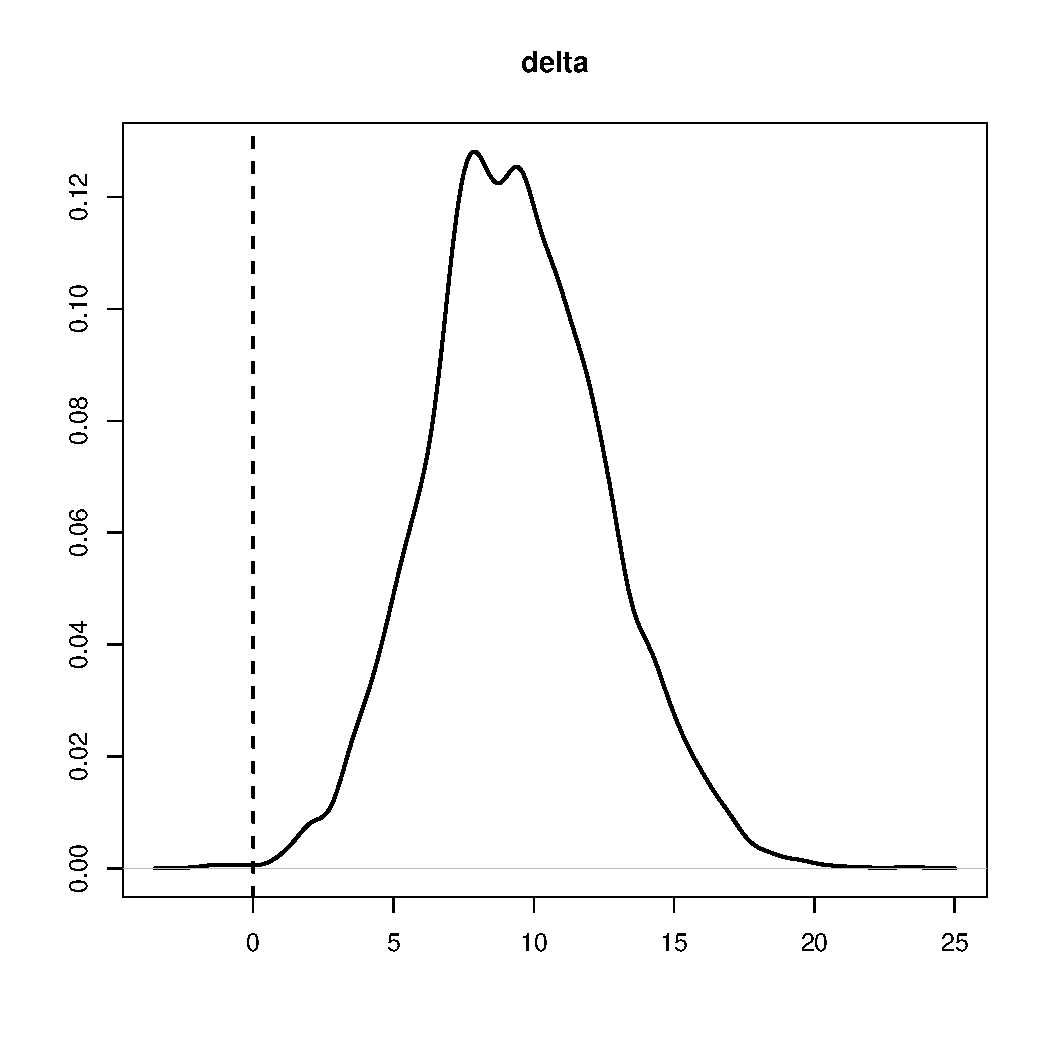
\includegraphics[width=.4\textwidth, height=.4\textheight]{\figfig/posterior-density-delta}
  $$
  
  \begin{center} {\tt \begin{tabular}{lrrrcr}
  & post.mean  & post.mode  & lower.CI  & upper.CI \\ 
  \hline 
  delta  & 9.389825  & 8.824822  & 3.539045  & 15.84367 
  \end{tabular} } \end{center}
}

%====================================================================
\frame{ \frametitle{Monte Carlo: Illustration (1/3)} \label{app:MCillustration}
  
  \paragraph{Example.} $\pi(\theta) = \Ncal(0, 10)$, $g(\theta) = e^\theta$:
  \begin{itemize}
   \item {\tt theta.sample = rnorm(M, mean=0, sd=sqrt(10))}
   \item {\tt mean(exp(theta.sample))}
%    \item   
%    \begin{tabular}{crrrrc}
%     $M$ & 1e3 & 1e4 & 1e5 & 1e6 & truth \\
%     \hline
%     $\widehat{\Esp}(g(\thetabf))$ & 388.27 & 140.06 & 133.08 & 170.40 & 148.41
%   \end{tabular}
  \end{itemize}
}

%====================================================================
\frame{ \frametitle{Monte Carlo: Illustration (2/3)}

  \paragraph{Properties.} 
  \begin{itemize}
   \item Easy to implement
   $$
    \text{\tt mean(exp(rnorm(M, mean=0, sd=sqrt(10))))}
   $$ \\~
   \item \pause Unbiased: $\Esp\left[\widehat{\Esp}(g(\thetabf))\right] = \Esp(g(\thetabf)$ \\~
   \item \pause Precision proportional to $1 / \sqrt{M}$ \\~
   \item \pause Still, very variant in practice (see next)
  \end{itemize}
 }

%====================================================================
\frame{ \frametitle{Monte Carlo: Illustration (3/3)}

  \begin{tabular}{cc}
    \begin{tabular}{p{.5\textwidth}}
     $
     \theta \sim \textcolor{blue}{\Ncal(0, 10)}, 
     \quad
     g(\theta) = \textcolor{red}{e^\theta}
     $
     
     \bigskip
    \begin{tabular}{lrr}
	 & mean  & sd \\ 
	 \hline 
	 1000  & 194.67  & 338.96 \\ 
	 10000  & 139.63  & 47.24 \\ 
	 1e+05  & 155.65  & 86.93 \\ 
	 1e+06  & 147.76  & 15.68 \\ 
	 truth  & 148.41  & -- 
	 \end{tabular}
    \end{tabular}
    & 
    \hspace{-.1\textwidth}
    \begin{tabular}{p{.5\textwidth}}
	 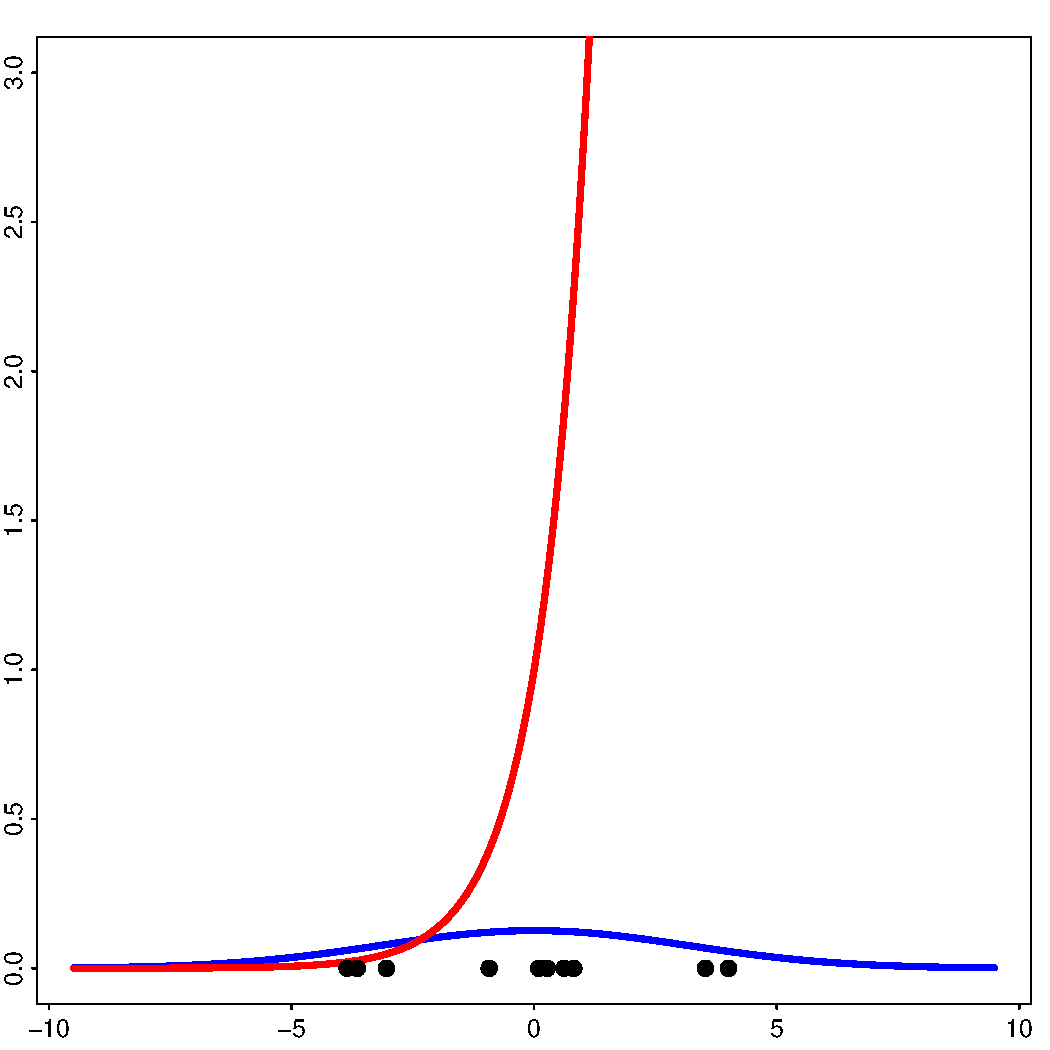
\includegraphics[width=.4\textwidth, height=.4\textheight]{../figs/EspLogNorm-MC} \\
	 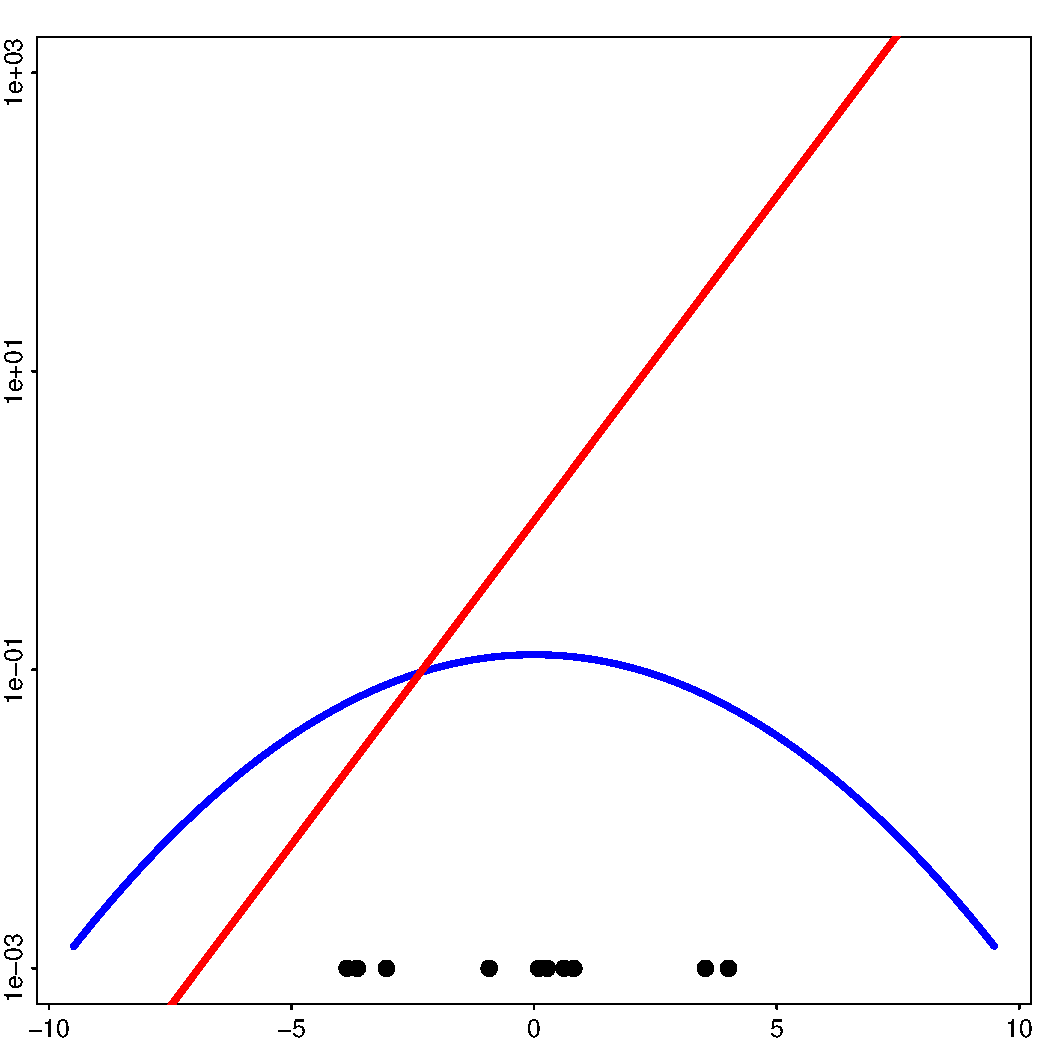
\includegraphics[width=.4\textwidth, height=.4\textheight]{../figs/EspLogNorm-MC-log} 	 
    \end{tabular}
  \end{tabular}
}



